\chapter{Background and Related Work}
\label{cha:background}

A large part of the work undertaken during this project requires a significant understanding on how a particular deep learning architecture, the Transformer works. In this section, we will cover some of the required background and insights drawn from the Transformer architecture which were needed to solve our problem.We can also refer to such a section~\ref{sec:background}.

\section{Background on Transformers}
\label{sec:background}


We will write this section similar to the section from the HotNets paper. More details on relevant transformers will be added, figures will be reused with credit as per required. Use~\ref{} where needed, zotero will export all of this.

We can also add a figure~\ref{fig:eth}.

\begin{figure}[!hbt]
  \begin{center}
    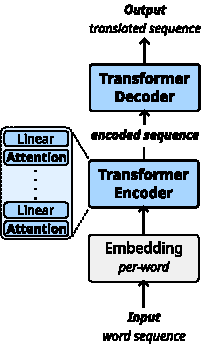
\includegraphics[width=0.5\textwidth]{figures/architecture_transformer.pdf}
    \caption{This is a sample image, credits: Alex}
    \label{fig:transformer}
  \end{center}
\end{figure}

Tables can also be useful.\footnote{%
Tips for beautiful tables: %
\url{https://texdoc.net/texmf-dist/doc/latex/booktabs/booktabs.pdf}}


\begin{table}[htbp]
\centering
\begin{tabular}{ c  p{130pt}  l }
\toprule
Column 1 & Column 2 \newline (additional line) & Column 3 \\
\midrule
C1,R2 & C2,R2 & C2,R3 \\
C1,R3	& \multicolumn{2}{ c }{C2\&C3,R3} \\
C1,R4 & C2,R4 & C3,R4\\
\bottomrule
\end{tabular}
\caption{Table 1}
\label{tab:table1}
\end{table}

\section{Related Work}
\label{sec:related_worl}

Is there much to add here? We claim that no one really tried to solve this problem as it was a "lost" cause. However, maybe some references such as MimicNet/Aurora can be added here added here, as we did look at them to an extent.

If we refer to another paper, book, website, \dots we add a
citation~\cite{Lamport:LaTeX}.
